\section{Market Analysis}
Identify target users or customers, user needs, existing products or 
solutions, competitors, market trends, and the market gap addressed 
by the project.

Our vacuum cleaner is primarily aimed at the european market. Therefore, the
following analysis is based surveys and predictions done on this market only, unless
otherwise specified.
\subsection{Projected Market Size and Growth}
According to a report by data bridge market research, the current robotic vacuum
cleaner market in Europe has a market size of about 1.65 billion $USD$ with a
compounding annual growth Rate (CAGR) of around 10 \% to a market size of around
3.39 billion $USD$\nomenclature{$USD$}{ United States Dollar} in 2032.\cite{market_analysis_1}

\begin{figure}[H]
    \centering
    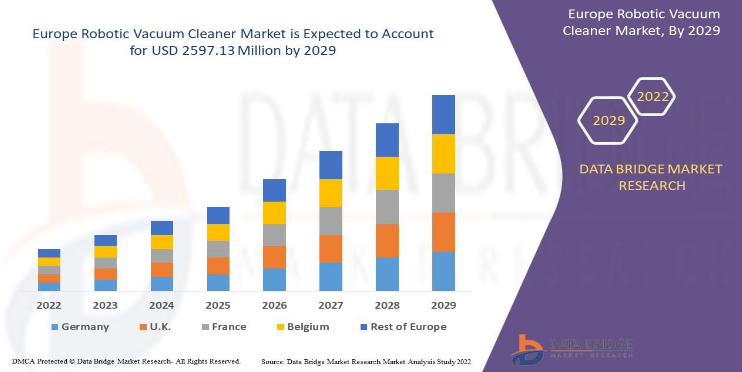
\includegraphics[width=0.7\textwidth]{images/market_analysis_1.png}
     \caption{Expected growth of the european market until 2032}
    \label{fig:marketanalysis_1}
\end{figure}

These numbers clearly indicate a flourishing market with lots of growth potential.
Out of all the robotic cleaners, the vacuuming floor robot is the most in demand and has
the biggest market share out of all the options.\cite{market_analysis_2}

\begin{figure}[H]
    \centering
    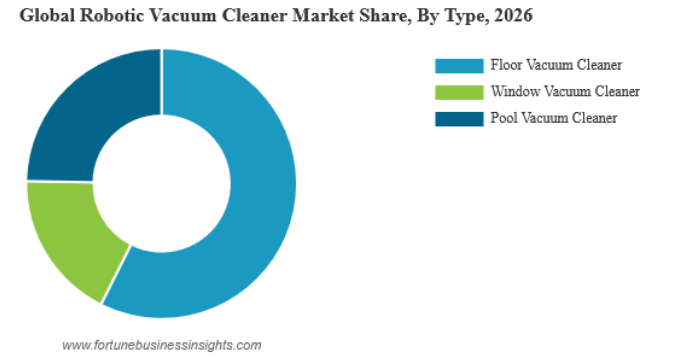
\includegraphics[width=0.7\textwidth]{images/market_analysis_2.png}
     \caption{Global Market Vacuum Cleaner Market Share}
    \label{fig:marketanalysis_2}
\end{figure}

\subsection{Most in demand robot type}
Another survey done by fortune also came to the conclusion that the robot type most in
demand is the class of robots below 150 $USD$.\cite{market_analysis_3}
Since we are building a prototype with a budget of 2000 $DKK$\nomenclature{$DKK$}{Danish Crowns} (around 300 USD), we are
confident that a successful prototype would mean that the final product is in this exact price category.


\subsection{User Analysis}
The primary target group for this vacuum robot prototype consists of young
professionals (aged 24–35) living in urban apartments ranging from 50 to 90 $m^2$. This
demographic is characterized by:

\begin{itemize}
    \item Demanding work schedules leaving less free time and consequently desiring an effortless way to clean the house without spending personal time on chores.
    \item High digital literacy, thus expecting everything to be operable via an app.
    \item Price sensitivity: possessing a limited budget and income and seeking an economical price point while still providing all essential functions.
\end{itemize}

As a result, our target group wants a straightforward way to keep their apartment clean
without investing their own time.
We are focusing on the bare minimum of cleaning functionality to keep costs as low as
possible, while still delivering necessary features (vacuuming and obstacle navigation)
and omitting luxury extras like self-emptying stations or camera recognition.
Since we can expect our demographic to be relatively digitally adept, we are integrating
numerous functions—such as starting and stopping the robot—into a mobile
application. This approach appeals directly to the consumer and allows us to turn
hardware constraints into smart software solutions.